\subsubsection{Fotoshoot UI}

Das Fotoshoot UI hat mehrere Funktionen. Es dient um den Ballwurf-Prozess zu starten, die Korberkennung zu kalibrieren und die Motoren anzusteuern.

\noindent
\textbf{Ballwurf-Prozess}
Der gesamte Prozess kann mittels dem Start-Knopf gestartet werden. Die Benutzeroberfläche wird eingefroren und die Zeit wird gestoppt. Sobald der Prozess beendet wurde, wird die vergangen Zeit angezeigt.

\begin{figure}[h!]
\centering
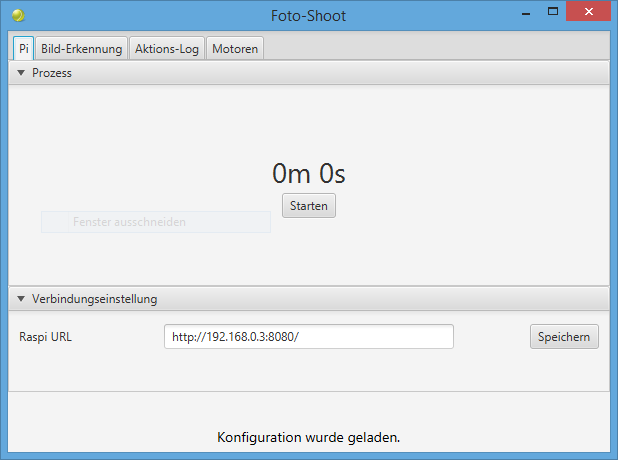
\includegraphics[width=0.7\linewidth]{../../fig/fotoshoot-ui/fotoshoot-ui-pi}
\caption{Fotoshoot-UI Prozess starten}
\label{fig:fotoshoot-ui-pi}
\end{figure}

\noindent
\textbf{Kalibrierung der Korberkennung}
In diesem Bereich können die Parameter für die Bild-Erkennung definiert werden. Die Bedeutung der Parameter sowie die gültigen Werte sind in Abschnitt \ref{sec:parameter-bild-erkennung} detailliert beschrieben.

\begin{figure}[h!]
	\centering
	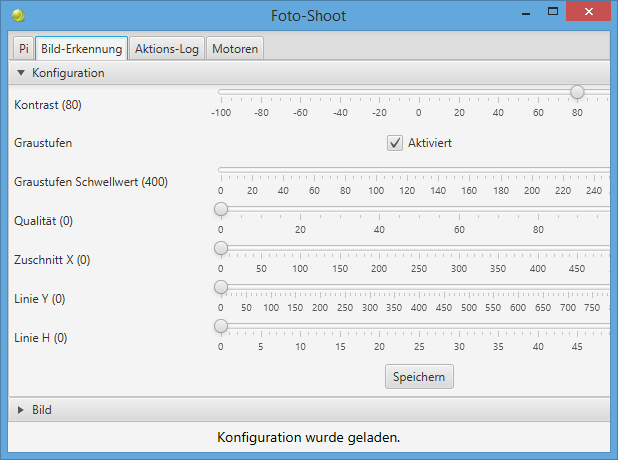
\includegraphics[width=0.7\linewidth]{../../fig/fotoshoot-ui/fotoshoot-ui-korb-erkennung}
	\caption{Fotoshoot-UI Bilderkennung}
	\label{fig:fotoshoot-ui-korb-erkennung}
\end{figure}

\noindent
\textbf{Ansteuerung der Motoren}
Die einzelnen Motoren können über die Benutzeroberfläche angesteuert werden. Dies vereinfacht das Testen der einzelnen Komponenten massiv und macht es auch für alle zugänglich. Es braucht nun kein spezielles IT-Know-How mehr um die einzelnen Komponenten zu starten.

\begin{figure}[h!]
	\centering
	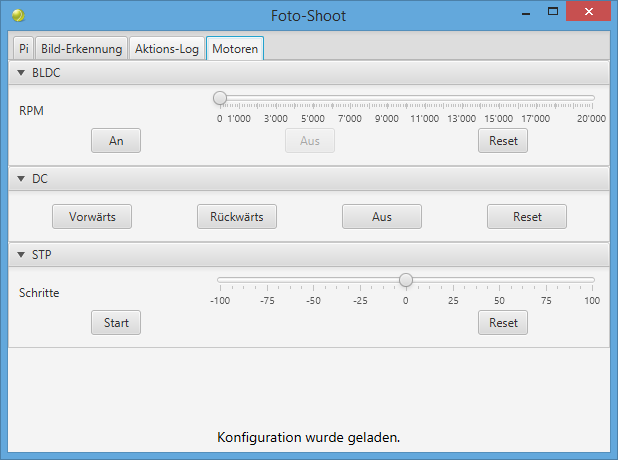
\includegraphics[width=0.7\linewidth]{../../fig/fotoshoot-ui/fotoshoot-ui-motoren}
	\caption{Fotoshoot-UI Ansteuerung der Motoren}
	\label{fig:fotoshoot-ui-motoren}
\end{figure}

\noindent
\textbf{Technische Umsetzung}
Das Fotoshoot-UI wurde in Java und mit der heute aktuellen UI-Technologie Java-FX implementiert. Zudem sind zentral zwei 3rd-Parties, welches den Bau dieser Applikation massiv vereinfachen soll.

\begin{itemize}
	\item Google Guice: Dies ist ein Depedency Injection Framework. Die Controller können nun ihre zusätzlichen Abhängigkeiten über die Injektion erhalten. Der Objekt-Baum muss nicht mehr mühsam von Hand erzeugt werden.
	\item Eventbus: Der Eventbus ist Teil von Google Guava. Dieser vereinfacht die Implementation des Observer-Patterns. Jeder kann auf den Eventbus Events senden und sich mit lediglich der Annotation @Subscribe für Events registrieren.
\end{itemize}
	
\begin{figure}[h!]
	\centering
	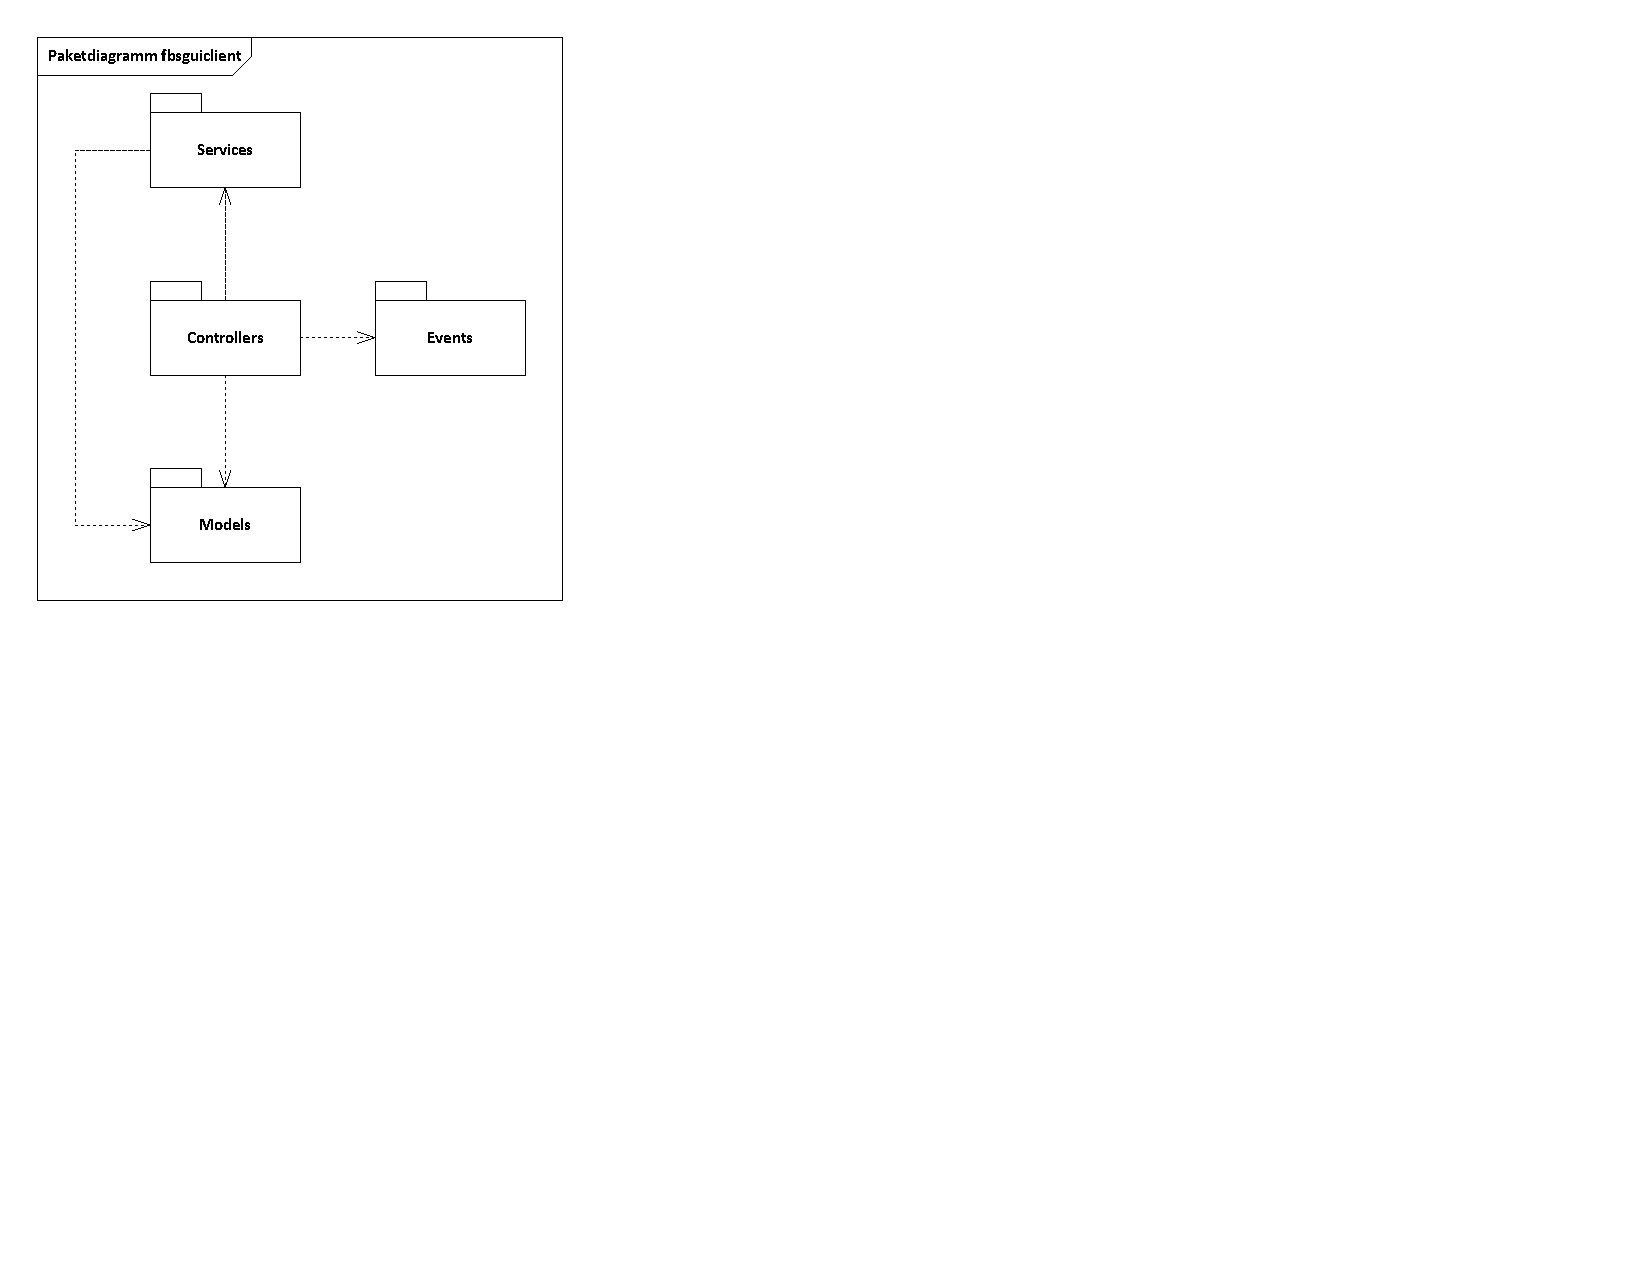
\includegraphics[width=0.7\linewidth]{../../fig/fotoshoot-ui/fotoshoot-ui-paketdiagramm}
	\caption{Paketdiagram Fotoshoot-UI}
	\label{fig:fotoshoot-ui-paketdiagramm}
\end{figure}
		
Auf der Abbildung \ref{fig:fotoshoot-ui-paketdiagramm} ist zu erkennen wie die Applikation aufgebaut ist. Nachfolgend werden die einzelnen Pakete erklärt:
		
\begin{itemize}
	\item Controllers: Die Controllers beinhalten die FXML-Dateien und die konkreten Controller Klassen. Controller sind für die Benutzer-Aktionen, Service-Calls, sowie die Beziehung zwischen Modell und UI zuständig.
	\item Modell: Dies sind die Modelle fürs GUI. Diese sind fürs GUI zugeschnitten. Die Modelle beinhalten die Properties, welche über die Controller in die Views gebunden werden.
	\item Services: Diese sind zuständig zuständig für die Daten. Sowohl Daten-Abfrage und auch Manipulation. Stellen die Schnittstelle zum Business-Layer dar.
	\item Events: Das sind POJOs, welche von den Controller verwendet werden. Diese werden für die Kommunikation der Controller untereinander über den Eventbus benötigt.
\end{itemize}
			
Jeder Controller kann der Ursprung für eine Benutzeraktion sein, welcher Einfluss auf irgendwelche welche Views hat. Diesen Views liegen auch wieder Controllers zugrunde. Damit nicht jeder Controller jeden anderen Controller kennen muss, verwenden wir hier den EventBus von Google. Jeder Controller wird automatisch registriert und kann über den Eventbus Events senden und sich für jedes Event auch wieder registrieren.
